\documentclass[10pt,a4paper]{article}
%\usepackage{simplemargins}
\usepackage[margin=2.5cm]{geometry}
%\usepackage[square]{natbib}
\usepackage{amsmath}
\usepackage{amsfonts}
\usepackage{amssymb}
\usepackage{graphicx}
\usepackage{easyReview}
\usepackage{caption}

\begin{document}
	\pagenumbering{gobble}
	
	\Large
	\begin{center}
		Enhanced Pedestrian Dead Reckoning Sensor Fusion for Firefighting\\ 
		
		\hspace{10pt}
		
		% Author names and affiliations
		\large
		Tobias Augustin, Daniel Ossmann \\
		
		\hspace{10pt}
		
		\small  
		Munich University of Apllied Sciences HM\\
		\{tobias.augustin, daniel.ossmann\}@hm.edu\\
		
		
	\end{center}
	
	\hspace{10pt}
	
	\normalsize
	
	Knowing a firefighters position in a building during an indoor attack is crucial to improve firefighting efficiency and safety. Since the commonly used GPS lacks the needed accuracy in indoor environments, an alternative solution is needed. Examples are Radio or Wi-Fi Triangulation or Magnetic Field Mapping. However, First Responders unique challenges call for an approach reliant solely on body-worn sensors. This approach, known as Pedestrian Dead Reckoning (PDR), estimates an individual's position relative to a starting point. Many PDR solutions utilize step detection as their main means of position tracking. While this produces accurate results during normal walking processes, during dynamic activities like crouching the accuracy is significantly lower. In this paper we propose an approach that features an enhanced sensor data fusion algorithm to increase position estimation accuracy. The algorithm features a robust step detection with a optical position tracking device as a secondary sensor. For this a body mounted Inertial Measurement Unit (IMU) and Tracking Camera are used. The measured velocity and position data is fused in an Extended Kalman Filter (see Figure 1). To evaluate the quality of the sensor fusion algorithm, tests are performed in a cage for unmanned aerial vehicle (UAV). The UAV cage allows a sub centimeter tracking resolution of an individuals position. With the enhanced sensor fusion, a mean error of less than $1\;\mathrm{m}$ can be achieved which is significantly lower than an approach based sole on step detection. Figure 2 shows the comparison between the algorithm using enhanced sensordata fusion and the step detection algorithm.
	\vspace{1cm}
	
	\begin{minipage}[l]{0.47\textwidth}
		\hspace*{-0.5cm}
		\vspace{-2cm}
		\begin{center}
			
			%\vspace{-2.3cm}
			%\hspace{-0.5cm}
			\includegraphics[width=1\textwidth]{Bilder/schema1.png}
			
			\captionof{figure}{Schematic structure of the enhanced sensorfusion algorithm. The position data estimated by the Tracking Camera and the Step Detection Algorithm are the measurement inputs of the Kalman Filter}
		\end{center}
		
	\end{minipage}
	\hspace{1cm}
	\begin{minipage}[r]{0.4\textwidth}
		\hspace{-0.5cm}
		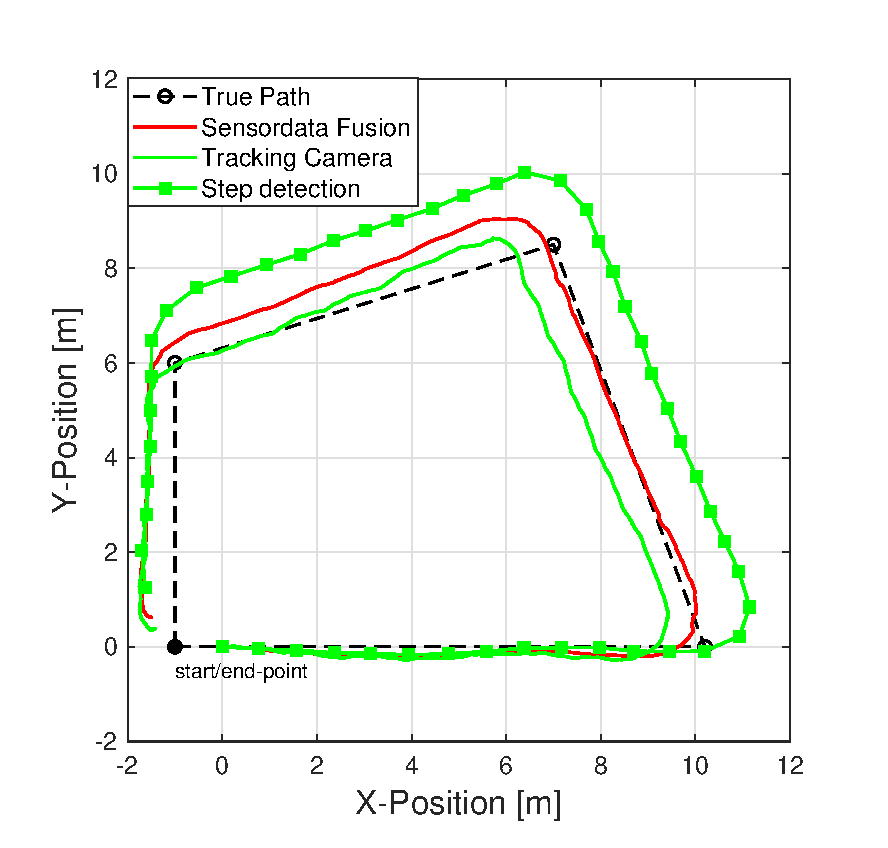
\includegraphics[width=1.2\textwidth]{Bilder/plotPaths.eps}
		
		\captionof{figure}{Comparison between Position Estimation based solely on a step length estimation algorithm or a Tracking Camera and the results estimated by the sensordata fusion algorithm.}
	\end{minipage}
	
\end{document}